\documentclass{mprop}
\usepackage{graphicx}
\usepackage{algorithm}
\usepackage{algpseudocode}
\usepackage{float}
\usepackage{siunitx}
\usepackage{xspace}
\usepackage{cite}
\graphicspath{ {images/} }

% alternative font if you prefer
% \usepackage{times}

% for alternative page numbering use the following package
% and see documentation for commands
\usepackage{fancyheadings}


% other potentially useful packages
\usepackage{amssymb,amsmath}
%\usepackage{url}
%\usepackage{fancyvrb}
%\usepackage[final]{pdfpages}

\begin{document}

%%%%%%%%%%%%%%%%%%%%%%%%%%%%%%%%%%%%%%%%%%%%%%%%%%%%%%%%%%%%%%%%%%%
\title{Probabilistic Topic Modelling to Reduce the Noise in Metabolomics}
\author{Arijus Pleska}
\date{Date of submission placed here}
\maketitle
%%%%%%%%%%%%%%%%%%%%%%%%%%%%%%%%%%%%%%%%%%%%%%%%%%%%%%%%%%%%%%%%%%%

%%%%%%%%%%%%%%%%%%%%%%%%%%%%%%%%%%%%%%%%%%%%%%%%%%%%%%%%%%%%%%%%%%%
\tableofcontents
\newpage
%%%%%%%%%%%%%%%%%%%%%%%%%%%%%%%%%%%%%%%%%%%%%%%%%%%%%%%%%%%%%%%%%%%

%%%%%%%%%%%%%%%%%%%%%%%%%%%%%%%%%%%%%%%%%%%%%%%%%%%%%%%%%%%%%%%%%%%

% Metabolomics
% Vision
\section{Introduction}
% To-do:
% - Mention Rogers' paper for the first attempt to use LDA in Metabolomics datasets

% Intro
% - ML in biology
% - Data patterns
% - Noise
\par This research proposal suggests an application of machine learning in biology. We intend to study the scans of low level biological entities in order to derive their patterns. To be more specific, we will be tackling a problem of noise. This issue of noisiness arise from the hardware limitation of the high precision data collection devices.   

% Metabolomics
% - Mass spectrometry
\par The application domain of this project is metabolomics -- a branch of computional biology. In brief, metabolomics is the scientific study of chemical processes which involve small molecules -- metamobilites. Ultimately, these chemical processes can be predicted by the features of metabolites. We intend to set the basis of our study on data sets acquired by \textit{mass spectrometry} (MS). By using this technique, we obtain the masses and intensities of metabolites within a sample of interest. This data representation is known as mass spectrum. Note that a different mass indicates different types of metabolites, whereas intensity suggests the level of concentration. Thereby, a mass spectrum is used to distinguish and visualise the observed metabolites. By deriving the formulae of specific metabolites types, we can induce patterns leading to the prediction of chemical processes. 

% The domain of vision
% - Expalanation how the scans of metabolites can be treated as images.
% - Visualisation of particular metabolites or metabolite patterns.
\par In the terms of machine learning applicability, we are looking into a problem of vision. The metabolites of some biological tissue are sequentially captured within regions of fixed size. Effectively, this process is generating an image: each scan is a pixel, therefore, the collections of scans produce an image. However, each pixel contains a large amount of metabolites, so the visualisation of these in a single image would be rather complex. Thereby, we can choose a specific metabolite type and produce pixels reflecting such metabolite activity. For a rigorous discussion on machine learning applications in metabolomics, the reader can consult the recent survey conducted by Alonso et al. \cite{Alonso-et-al}. Going back to the visualisation of metabolites, we can choose a specific combination (structure) and produce an image where activated pixels would suggest the concentration of the chosen metabolite structure. The problem arises upon discovering valid matabolite structures. Therefore, the techniques of machine learning, or more specifically topic modelling, are used to induce the prospective structures.

% Unsupervisder learning
% - Topic moels
% - Probabilistic models
% - LDA:
% -- General
% -- Metabolomics
\par The objective to discover novel structures is treated as a problem of \textit{unsupervised} machine learning. That is, we have no initial settings in how these structures are expected to look like: the structures will be inferred by machine learning methodology. The inference of unknown structures is studied within \textit{topic modelling}. Further, note that we are concentrating on statistical topic modelling. In other words, we are putting the emphasis on the \textit{probabilistic} models: the structures are inferred from the data instance distributions. To be more specific, we are focusing to enhance a particular probabilistic machine learning model -- \textit{latent Dirichlet allocation} (LDA). First of all, the successor LDA models are treated as a state-of-the-art method in tackling semantic-analysis type problems. For more detailed review on the LDA applications, the reader can consult the survey \cite{blei_2012} conducted by Blei. Further, Hooft et al. \cite{hooft} has recently addressed the applicability of LDA in metabolomics. Note that this proposal is directly influenced by the latter prospect: we will attempt to utilise the LDA-like models to reduce the impact of noise in the data sets of the metabolomics domain.  

% Outline
% - Sections
\par The structure of this proposal is given as follows: in Section 2 we present the issue of noise in Metabolomics; in section 3 we cover the literature in topic modeling which focuses on the variations of Latent Dirichlet Allocation; in Section 4 we provide the metric of success of the proposed research; finally, in Section 5, we go into details on how the project will be executed.
% To-do: rewrite the outline

%%%%%%%%%%%%%%%%%%%%%%%%%%%%%%%%%%%%%%%%%%%%%%%%%%%%%%%%%%%%%%%%%%%%%%%%%
%%%%%%%%%%%%%%%%%%%%%%%%%%%%%%%%%%%%%%%%%%%%%%%%%%%%%%%%%%%%%%%%%%%%%%%%%
%%%%%%%%%%%%%%%%%%%%%%%%%%%%%%%%%%%%%%%%%%%%%%%%%%%%%%%%%%%%%%%%%%%%%%%%%
\section{Statement of Problem}

% Intro
% - Suggesting an advance in processing rather than equipment.
\par Currently, MS equipment is incapable to fully represent the metabolite construction. As discussed by Palmer et al. \cite{palmer}, even though the current machinery differentiates metabolites in millidalton precision, we still obtain a significant amount of false positives. Thereby, rather than relying upon the advances of MS equipment, we can investigate the prospect of enhancing the data processing techniques. As described in Section 1, LDA derivatives are promising methods in discovering the hidden structures in metabolomics data sets. For this reason, we raise a hypothesis that the degeneracies of metabolomics data sets can be detected using LDA-like models. Note that currently there is no set approach on how to configure LDA-like models to reduce the impact of noise in metabolomics data sets.  

% Objectives
% - Research in the state-of-the-art methodology.
% - Reducing the impact of noise in metabolomics.
% - Providing a general-purpose machine learning model.
\par The primary goal of this research is to expand the consensus on whether topic modelling is a valid approach to smooth metabolomics data sets. To be more specific, we set our objectives to the following:
\begin{enumerate}
    \item Utilise general topic modelling methods in metabolomics;
    \item Reduce the impact of noise in metabolomics data sets;
    \item Give a basis to a general topic modelling method for error correction.
\end{enumerate}
Briefly, the first objective is expected to utilise the general state-of-the-art topic modelling methodology to distinguish the techniques displaying better performance in metobolomics applications. In other words, we will conduct a survey on LDA-like topic modelling methodology. The second objective is focusing on enhancing the general models for the particular task of error correction in metabolomics. Finally, the third objective can be treated as a general contribution to the field of machine learning, since the discovered techniques might be applicable to other domains. 

% Hypothesis
% - Topic modelling can improve the quality of metabolomics data sets.
% - The negation of the hypothesis would contribute in terms of reassessing the complexity of the problem.
\par We are setting a hypothesis that LDA-like topic modelling can be successfully utilised to correct errors in metabolomics data sets. Both cases of proving and disproving this hypothesis would contribute to metabolomics. The successful outcome would lead to the potential applications discussed in the following paragraph, whereas the unsuccessful outcome would set-up additional requirements to tackle the issue of noisiness in metabolomics data sets.

% Results: tools to annotate the metabolites > basis for generative error correction 
% - Expanding the application of existing machine learning models.
% - Advancing the current state-of-the-art in metabolomics.
% - Contributing to machine learning in general.
\par The potential applications of this research can be directly induced from the previously listed objectives. First of all, we would show that the general models or the models applied in other domains can be utilised in metabolomics. Further, the developed error correction methodology would improve the accuracy of the chemical processes prediction. Finally, the generalisation of the developed error correction model might suggest different approaches in tackling error correction in general; also, it would impact the awareness in metabolomics and the field's potential in developing machine learning generalisations.  

%%%%%%%%%%%%%%%%%%%%%%%%%%%%%%%%%%%%%%%%%%%%%%%%%%%%%%%%%%%%%%%%%%%%%%%%%
%%%%%%%%%%%%%%%%%%%%%%%%%%%%%%%%%%%%%%%%%%%%%%%%%%%%%%%%%%%%%%%%%%%%%%%%%
%%%%%%%%%%%%%%%%%%%%%%%%%%%%%%%%%%%%%%%%%%%%%%%%%%%%%%%%%%%%%%%%%%%%%%%%%
\section{Background Survey}

% Intro
% - The reason why the literature review is conducted.
% - Outline: preliminaries, notation, literature.
% - A notification the the results will be discussed in the following section.
\par The provided literature review on topic modelling is directed towards familiarising with LDA derivatives. Also, the review assesses the methodology of LDA-like models and proposes several implementation variations. The review is structured in progressing order: at the start, we look into the original LDA paper and define the terminology (it will be used throughout the proposal); then, we familiarise with two different techniques used for the inference of LDA-like models; finally, we review LDA derivatives which shows the potential to be utilised in designing the error correction technique.

%%%%%%%%%%%%%%%%%%%%%%%%%%%%%%%%%%%%%%%%%%%%%%%%%%%%%%%%%%%%%%%%%%%%%%%%%
%%%%%%%%%%%%%%%%%%%%%%%%%%%%%%%%%%%%%%%%%%%%%%%%%%%%%%%%%%%%%%%%%%%%%%%%%
\subsection{Terminology}

% General intuition on topic modelling
% - Example
\par Recall that in topic modelling induces a hidden structure within the studied data sets. We will provide an example providing an intuition in this process. Say, if we were analysing a book, its chapters might address different topics or address the topics at a different extent. Further, the chapters itself would have unique distributions of the topics. Note that we are assuming that we do not know what the topics addressed in the book. In order to derive these hidden topics, a probabilistic topic modelling method would analyse the structure of the words used in the book. In other words, the model would induce patterns which would refer to a particular topic. Regarding the method's performance, it would depend on the method's ability to optimise the inference of the patterns. For example, commonly used words (such as and, or, the, etc.) would be relevant in all topics. Therefore, their semantic impact in defining the topics would be negligible. For this reason, we could dismiss these to improve the time performance of the method. 

% LDA intro
% - the model
% - A notification that the terminology and the notation will be useful throughout the proposal.
\par The terminology used in this proposal is equivalent to the terminology used by Blei \cite{blei_2012}. Figure \ref{fig:lda} below represents the original LDA model in plate notation. We will use it as a guide to familiarise with the terminology.   
\begin{figure}[H]
  \centering
  \includegraphics[width=0.7\textwidth]{lda_model}
  \caption{The design of the original LDA model}
  \label{fig:lda}
\end{figure}

% High level LDA terminology
% - Notation:
% -- List LDA definitions
% -- Explain the definitions
\par To start with, we will familiarise with the higher level entities of the model. The circles represent an entity, whereas the plates indicate the number of entities. For example, there would $N \times M$ entities of $z$ and $M$ entities of $\theta$. Further, LDA is a three-level hierarchical structure: the smallest entity (grey circle) is defined as a \textit{word}; then a collection of words (inner plate) is defined as a \textit{document}; and a collection of documents (outer plate) is a \textit{corpus}. Note that Figure 1 represents $M$ documents and $N$ words per document, it follows that in the corpus there would be $M \times N$ words. Also, as suggested by Figure 1, let's denote a word by $w$. Then, let's denote the sequence of words in document $d$ by 
\begin{equation*}
\mathbf{w}_d = \{w_1, w_2, \dots, w_N\},
\end{equation*}
then the sequence of words in the corpus would be denoted by
\begin{equation*}
\mathcal{\mathbf{D}} = \{\mathbf{w_1}, \mathbf{w_2}, \dots, \mathbf{w_M}\}.
\end{equation*}
 
% Low level LDA terminology
% - Intro to observable and hidden variables
% - Notation:
% -- List the definitions
% -- Explain the definitions
\par Now, we will introduce the lower level entities. The grey circle indicates that the \textit{observable} variables, whereas the white coloured circles indicate the \textit{hidden} variables. Note that in Figure 1 the words are the only observable variables; all other entities are hidden, i.e., they describe the underlying structure of the model. Further, recall that topic modelling is applied in order to discover a mixture of topics; or in other words, topic modelling could describe a corpus and its documents in terms of topic distributions. This intuition will simplify the definitions of the remaining entities in Figure 1, these are given as follows:
\begin{itemize}
\item $K$ is the number of topics;
\item $V$ is the size of the vocabulary, i.e. the number of unique words in the corpus;
\item $\alpha$ is the parameter referring to the prior distribution of the topics over documents;
\item $\beta$ is the parameter referring to the prior distribution of the vocabulary over topics;
\item $\theta$ is the latent variable referring to the topic distribution over documents;
\item $\phi$ is the latent variable referring to the vocabulary over topics
\item $w$ is the observable variable referring to the words in documents;
\item and $z$ is the latent variable of topic assignments over the words.
\end{itemize}
Further, note that the listed entities can be perceived as matrices of the following dimensions: $\alpha$ is $1 \times K$; $\beta$ is $K \times V$; $\theta$ is $M \times K$; $\phi$ is $M \times K$; $w$ is $M \times N$; and $z$ is $M \times V$.
% To-do: check the dimensions

%%%%%%%%%%%%%%%%%%%%%%%%%%%%%%%%%%%%%%%%%%%%%%%%%%%%%%%%%%%%%%%%%%%%%%%%%
%%%%%%%%%%%%%%%%%%%%%%%%%%%%%%%%%%%%%%%%%%%%%%%%%%%%%%%%%%%%%%%%%%%%%%%%%
\subsection{Preliminaries}

% Basic LDA
% - Generative process
% - The derivation of the posterior
\par The relationship the between observable and hidden variables, effectively, describes the inference of the underlying topic structure. We will go through an arbitrary example in order to give an intuition in the inference process and familiarise with the lower level notation of the previous listed variables. Figure \ref{fig:lda} shows see that $\alpha_k$ (the prior for the $k$th topic in a document) influences $\theta_{:, k}$ (the latent variable describing the distribution of topic $k$ over all documents). It follows that $\theta_{d, k}$ (the probability of the $k$th topic occurrence in document $d$) influences $z_{d, :}$ (the topic assignment over all vocabulary terms for document $d$). Further, $z_{d, v}$ refers to the topic assignment of vocabulary term $v$. By taking $z_{d, v}$ and $\beta_{v, k}$ (the prior of topic $k$ on vocabulary term $v$), we obtain word $w_{d, v}$. In the complete perspective, the generative process of the corpus is given by the following joint probability distribution
\begin{equation}
p(\beta, \theta, z, w) = \prod_{k=1}^Kp(\beta_{:, k})\prod_{d=1}^Dp(\theta_{d, :})\bigg(\prod_{v=1}^Vp(z_{d, v} | \theta_{d, :})p(w_{d, v} | \beta, z_{d, v})\bigg).
\end{equation}
By using Bayes Theorem, we derive the computation of the conditional distribution
\begin{equation}
p(\beta, \theta, z | w) = \frac{p(\beta, \theta, z, w)}{p(w)}. 
\end{equation}
This equation expresses the computation of the posterior -- the derivation of the hidden corpus structure given observable variable $w$. The problem arises from inefficient analytical computation of evidence $p(w)$. The approximation of it will be considered during the literature review on LDA-like models. The naming of the following subsections corresponds to the reviewed papers. 

%%%%%%%%%%%%%%%%%%%%%%%%%%%%%%%%%%%%%%%%%%%%%%%%%%%%%%%%%%%%%%%%%%%%%%%%%
%%%%%%%%%%%%%%%%%%%%%%%%%%%%%%%%%%%%%%%%%%%%%%%%%%%%%%%%%%%%%%%%%%%%%%%%%
\subsection{Latent Dirichlet Allocation}

% Intro
% - Detailed approach in covering implementations details
\par Latent Dirichlet allocation is a probabilistic topic modelling technique proposed by Blei et al. \cite{blei_2003}. Since this paper is the origin of LDA-like models, it will be discussed in more detail to introduce the basis of LDA-like methodology. As a result, this coverage will simplify the review on the LDA derivatives discussed in the upcoming subsections. 

% Assumptions 
% - Bag of words principle
% - Discrete data sets
% - Topic dimensionality
\par The original LDA model sets some assumptions for the data processed by the model. First of all, it is assumed that documents and words are \textit{exchangeable}. That is, the order in which these entities are processed does not matter. In other words, we can say the model follows the \textit{bag-of-words} principle. The next assumption states that we should use discrete data. Effectively, the basic LDA does not cover  continuous features. Another assumption is on the number of topics: it is set to be fixed throughout the complete run of inference.  

% Generative process
% - Three level hierarchy
% - The generative algorithm
\par As discussed in the preliminaries subsection, we are also taking an assumption that the corpus is induced by a probabilistic process. The generation of the corpus has three levels: the parameters $\alpha$ and $\beta$ are sampled once; the variable $\theta$ is sampled once per document; and the variables $z$ and $w$ are sampled once per word. This hierarchical process relates to the generative algorithm given in the original LDA paper, it is equivalent to Algorithm 1 below.
\begin{algorithm}[H]
\caption{Document Generation}
\label{alg:document_generation}
\begin{algorithmic}[1]
\State $N \sim \mbox{Poisson}(\xi)$
\State $\theta \sim \mbox{Dir}(\alpha)$
\For {$n \leftarrow 1, N$}
\State $z_n \sim \mbox{Multinomial}(\theta)$
\State $w_n \sim \mbox{p}(w_n | z_n, \beta)$
\EndFor
\end{algorithmic}
\end{algorithm}
Note that the algorithm describes the generation of a single document. In order to generate the whole corpus, we would run the algorithm for each document. Going back to Algorithm 1, a brief intuition behind it is given as follows: in line 1 we draw the number of words $N$ in a document ($\xi$ is an ancillary variable used as the mean for the Poisson Distribution); in line 2 we draw topic distribution $\theta$ from the Dirichlet distribution on parameter $\alpha$; further, in lines 3--6 we generate the words: in line 4 we draw topic $z_n$ from the multinomial distribution on $\theta$ and, finally, in line 5 we obtain  word $w_n$ from the conditional probability on $z_n$ and $\beta$, recall that $\beta$ is the prior on the vocabulary terms correspondence to topics.


% Variational inference 
% - Variational parameters gamma and fi
\par As suggested in the ending paragraph of the preliminaries subsection, the inference relates to the computation of evidence $p(w)$ (it is the denominator term given in Equation 2). Even though the original paper mentions the inference methods such as Markov chain Monte Carlo, it suggests using the method of variational inference. In order to develop an intuition over the method, the authors introduce the variational parameters $\gamma$ and $\phi$. It is also mentioned that the computation of $\gamma$ and $\phi$ is an optimisation problem. That is, we are assessing the minimum bound over the latter parameters. Further, recall that in Figure 1 we explicitly express the parameter $\phi$ in describing the basic LDA model. However, the authors have chosen to show it separately -- upon describing the variational method. Their expression is given in Figure \ref{fig:var_par} below.
\begin{figure}[H]
  \centering
  \includegraphics[width=0.4\textwidth]{variational_parameters}
  \caption{Variational parameters}
  \label{fig:var_par}
\end{figure}
Note that the authors provide pseudo code to build an intuition in tackling this optimisation problem.

% Parameter estimation
% - M-step is an update of beta
% - Newton--Raphson is used to update alpha
% - The smoothing issue: 
% -- Sparsity from large data sets
% -- The incoorperation of documents which were not used for the training
\par Additionally, the authors emphasise the estimation of the parameters $\alpha$ and $\beta$. They use a two-step EM procedure which involves the previously introduced variational parameters $\gamma$ and $\phi$. E-step is the solution of the variational parameters optimisation problem; and M-step is an update of the parameters $\alpha$ and $\beta$. Note that the authors provide an analytical approach to estimate $\beta$ which is proportional to the changes of $\phi$; and for $\alpha$, they provide an approach utilising the Newton--Raphson method. Apart from that, the authors introduce the an issue of \textit{sparsity} in a corpus structure. A sparse corpus is expected upon using a large vocabulary or a large amount of documents. This issue is addressed by introducing smoothing: an additional parameter $\eta$ is utilised to smooth the estimation of $\beta$. 

% Experiments
% - Document modelling: issue with pLSI and mixture unigrams~ 
% - Document classification: 
% -- Dimensionality reduction
% -- Comparison with SVM
\par The conducted experiments display an improvement in performance over the predecessor models and suggest the application domains of LDA-like models. The first experiment addresses document modelling. LDA  has displayed balanced hidden topic proportions in the set of tested documents. That is, the tested documents has replicated the topic proportions of the training documents. The second experiment is directed towards the problem of document classification. They have addressed the \textit{dimensionality reduction} in order to surpass the performance of the support-vector-machine-like models. To be more specific, the documents with reduced dimensionality would possess a lower amount of features. The results of the experiment indicate that the basic LDA model has successfully reduced the number of features. Also, it has displayed an improvement in accuracy compared to the support-vector machine-like model. 
% To-do: explain perplexity (UNTOUCHED)

% Conclusion
% - Summary of the results established by the paper
\par The review on the original LDA model has set up a basis required to understand the model's derivatives. That is, the introduced methodology will be useful in considering the following improvements: (1) the  relaxation of the exchangeability assumption; (2) the adaptation of time-series suggesting word correspondence to topic over time; (3) the discussion over alternative inference methods. Apart from that, the experiments introduced in this section has reflected the LDA performance upon the model's introduction to the public. The current state-of-the-hard topic modelling techniques overcome the shown results. The experiments were addressed in order to suggest the application fields of LDA-like models.
% To-do: rework the paragraph name to reflect its purpose: remove the discussion (you might think it's done, but it's not)

%%%%%%%%%%%%%%%%%%%%%%%%%%%%%%%%%%%%%%%%%%%%%%%%%%%%%%%%%%%%%%%%%%%%%%%%%
%%%%%%%%%%%%%%%%%%%%%%%%%%%%%%%%%%%%%%%%%%%%%%%%%%%%%%%%%%%%%%%%%%%%%%%%%
\subsection{Finding Scientific Topics}

% Intro
% - Sampling as a method of inference
\par The paper on "Finding scientific topics" [CITATION] suggests an alternative approach to the inference in latent Dirichlet allocation. To be more specific, the paper provides a readable introduction on how to apply a Markov chain Monte Carlo (MCMC) algorithm as a sampling-based method for the inference in topic modelling. Further, the authors discuss the method's application settings in vision and conduct an experiment on deriving topics from the abstracts of papers published in "Proceedings of the National Academy of Sciences" (PNAS). Finally, the authors compare the performance of the suggested sampling-based inference method to variational inference methods. 

% Gibbs Sampling
% - Recall the meaning of phi and theta.
% - Introduce the inference method
\par The inference method using a Markov chain Monte Carlo algorithm can be referred by \textit{Gibbs sampling}. The authors claim that the method provides a first-order approximation in deriving the topics on the given corpus. That is, we can establish quantitative reasoning on the document correlation in terms of content and content's change over time. Recall that by $\theta$ we denote the topic distribution over documents and by $\phi$ we denote the topic distribution over words. In Gibbs sampling, these values can be obtained by examining the posterior distribution. Essentially, the variables are sequentially sampled from their respective distributions. The process draws topic assignment $z_i$ and keeps a track of this assignment with respect to each word and document. Note that $z_i$ is drawn from the following distribution:
\begin{equation}
P(z_i = j | z_{-i}, w) \propto \dfrac{n_{-i, j}^{(w_i)} + \beta}{n_{-i, j}^{(\cdot)} + W\beta}\dfrac{n_{-i, j}^{(d_i)} + \alpha}{n_{-i, \cdot}^{(d_i)} + T\alpha}.
\end{equation}
It follows that this distribution is utilise the previously mentioned topic assignments. For a brief familiarisation with the notation used in the previous expression, note the following: $n_j^{d}$ and $n_j^{w}$ are the counts of topic $j$ assignments in document $d$ and word $w$; $W$ is the number of words; and $T$ is the number of topics. Ultimately, the left side of the expression is $\phi$ and the right side is $\theta$. That is, 
\begin{align*}
\phi_j &= \dfrac{n_{-i, j}^{(w_i)} + \beta}{n_{-i, j}^{(\cdot)}},\\
\theta_j &= \dfrac{n_{-i, j}^{(d_i)} + \alpha}{n_{-i, \cdot}^{(d_i)} + T\alpha}.
\end{align*}
This process of topic assignment would be executed for every word in a document and for all documents in the corpus. The procedure would be repeated until the distributions displayed fluctuations below some set threshold. Notice that the procedure does not require direct assignment of $\theta$ and $\phi$. If needed, the values of these can be sampled upon converge by using the previously provided representations.

% Auxilliary xperiments
% - Vision
% - Time series
\par The authors have executed Gibbs sampling in the domain of vision. They have represented an image as a document and each pixel as a word. This means that they were able to recover the underlying basis from which the images could be constructed. The performance was compared to the latent Dirichlet allocations models which use variational inference. Note that we define the performance in terms of perplexity, which indicates the uncertainty of the word assignment to a topic. It appears that, with relatively small data sets, Gibbs sampling displays superior performance. Further, the authors have investigated the performance upon varying the number of topics. The results indicate that there exists a trade-off between the model being able to cover the significant underlying topics (low number of topics) and start deriving irrelevant branches (high number of topics).

% The main experiment
% - PNAS
\par The main experiment was carried in the PNAS data set, note that the processed papers were published from 1991 to 2001. By having a varying notion of time, the authors were able to investigate the prevailing topics. Thus, establish a sense in dynamic topic modelling. Even though the model was not adjusted to smooth the time-series, from the derived results we can deduce the varying relevance of underlying science domains.  

% Conclusion
\par We have reviewed an alternative method for the inference in latent Dirichlet allocation. The idea behind the inference process was explained by considering the primary aspects: the notion of counts and the implicit use of hidden variables. Also, we have introduced the experiment settings its results. This allowed to familiarise with an example of topic modelling application and vision. Further, the experiment on PNAS has emphasised the relevance of time series

%%%%%%%%%%%%%%%%%%%%%%%%%%%%%%%%%%%%%%%%%%%%%%%%%%%%%%%%%%%%%%%%%%%%%%%%%
%%%%%%%%%%%%%%%%%%%%%%%%%%%%%%%%%%%%%%%%%%%%%%%%%%%%%%%%%%%%%%%%%%%%%%%%%
\subsection{Dynamic Topic Models}

% Intro:
% - Time series
% - Qualitative and quantitative improvement
\par Now we review the paper on Dynamic Topic Models [CITATION]. Effectively, the dynamic topic model can be treated as an extension of static topic models (such as latent Dirichlet allocation). The main idea behind a dynamic topic model is that it induces the topic evolution the processed corpus. That is, the documents in the corpus evolve over time. In this subsection, we review the key assumptions of dynamic topic models, go over the generative process of documents, review the suggested inference methods, and familiarise with the results of the carried experiment. 

% Assumptions
% - Data is divided in time slices
\par We will emphasise the assumptions given on the dynamic topic models. First of all, even though we are discussing a model of time series suggesting the use of continuous variables, the data remains categorical. The distinction between continuous and categorical data is that continuous data is strictly numeric and infinite, whereas categorical data can take only particular values. The second assumption relaxes the ex-changeability on documents. That is, the documents are expected to form a sequence. Or in other words, the corpus is divided into time-slices. Note that in such time-slice documents are exchangeable.  

% Generative Process
% - Algorithm
% - An explanation of the algorithm
\par The generative process of the models updates the parameters $\alpha$ and $\beta$. This means that the topic distributions over documents and words change over time. The visualisation of the process is given in Figure 2 below.
\begin{figure}[H]
  \centering
  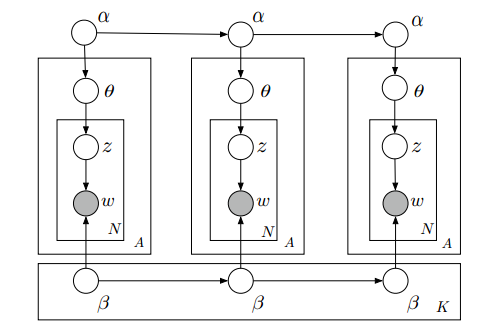
\includegraphics[width=0.7\textwidth]{dynamic_topic_model}
  \caption{Dynamic topic model. COPYRIGHT.}
  \label{fig:dtm}
\end{figure}
Notice that each time-slice is equivalent to the model shown in Figure 1. Also, the parameters $\alpha$ and $\beta$ are induced by their predecessors in the previous time-slice. More formal representation of the generative process is given in Algorithm 2. 
\begin{algorithm}[H]
\caption{Dynamic document generation.}
\label{alg:dynamic_document_generation}
\begin{algorithmic}[2]
\State $\beta_t | \beta_{t-1} \sim \mathcal{N}(\beta_{t-1}, \sigma^2)$
\State $\alpha_t | \alpha_{t-1} \sim \mathcal{N}(\alpha_{t-1}, \delta^2)$
\For {$d \leftarrow 1, D$}
\State $\eta_d \sim \mathcal{N}(\alpha_{t}, a^2)$
\For {$n \leftarrow 1, N$}
\State $z_{d, n} \sim \mbox{Multinomial}(\pi(\eta_d))$
\State $w_{t, d, n} \sim \mbox{Multinomial}(\pi(\beta_t | z_{d, n}))$
\EndFor
\EndFor
% \EndProcedure
\end{algorithmic}
\end{algorithm}
The given algorithm describes the generative process for the time-scale $t$. It starts by drawing the parameters $\alpha_t$ and $\beta_t$ from the Gaussian distribution with the means given by the previous parameter values. For now, we will not discuss the meaning of the variance values. Further, for each document in the time-scale, we carry the following procedure: we draw the topic distribution in a document $\eta_d$ from the Gaussian distribution with the mean given by $\alpha_t$; then, for each word in the document, we draw the topic $z_{d, n}$ from the Multinomial distribution on the parametrised $\eta_d$, and, finally, we draw the word $w_{t, d, n}$ from the Multinomial distribution on the parametrised $\beta_t$ which is conditioned on $z_{d, n}$. By the use of \textit{parametrisation}, we are expressing the result of the Gaussian distributions into a format suitable for Multinomial distribution. This mapping is expressed as
\begin{equation}
\pi(x)_n = \dfrac{\exp{(x_n)}}{\sum^n_{i=1}\exp{(x_i)}}.
\end{equation}

% Inference
% Variational methods are a deterministic alternavive for stochastic simulation
% Two variations: Kalman filtering and wavelet regression
\par The authors suggest using variational methods to approximate the inference posterior. It is claimed that stochastic simulation would be unable to scale with large data sets. Two techniques of variational methods are provided: Kalman Filtering and Wavelet Regression. The implementation details of these are provided in a brief manner suggesting the computation of the parameter $\beta_t$. 

% Experiments
% - Evolution of Science
\par The dynamic topic model is evaluated by conducting an experiment on the journals of \textit{Science}. The experiment is expected to establish the time series on the topic development with the articles. Indeed, the experiment is able to produce results displaying the rises and falls of the topics indicating scientific fields. Note that the experiment is performed using both variational inference methods.   

% Conclusion
\par The review on the dynamic topic models has familiarised us with more realistic generative process: the documents are induced by time series. Further, we have provided the visualisation of the model and introduced the algorithm for the generative process. Also, we have captured the techniques used for inference. Finally, we have familiarised with the experiment settings. 

% Section Conclusion
\par

%%%%%%%%%%%%%%%%%%%%%%%%%%%%%%%%%%%%%%%%%%%%%%%%%%%%%%%%%%%%%%%%%%%%%%%%%
%%%%%%%%%%%%%%%%%%%%%%%%%%%%%%%%%%%%%%%%%%%%%%%%%%%%%%%%%%%%%%%%%%%%%%%%%
%%%%%%%%%%%%%%%%%%%%%%%%%%%%%%%%%%%%%%%%%%%%%%%%%%%%%%%%%%%%%%%%%%%%%%%%%
\section{Proposed Approach}

% Section intro
\par

%%%%%%%%%%%%%%%%%%%%%%%%%%%%%%%%%%%%%%%%%%%%%%%%%%%%%%%%%%%%%%%%%%%%%%%%%
%%%%%%%%%%%%%%%%%%%%%%%%%%%%%%%%%%%%%%%%%%%%%%%%%%%%%%%%%%%%%%%%%%%%%%%%%
\subsection{Overview}

% Discussion over the literature
\par

%%%%%%%%%%%%%%%%%%%%%%%%%%%%%%%%%%%%%%%%%%%%%%%%%%%%%%%%%%%%%%%%%%%%%%%%%
%%%%%%%%%%%%%%%%%%%%%%%%%%%%%%%%%%%%%%%%%%%%%%%%%%%%%%%%%%%%%%%%%%%%%%%%%
\subsection{Approach}

% Design
\par

% Implementation
\par

% Evaluation/Experiments
\par

%%%%%%%%%%%%%%%%%%%%%%%%%%%%%%%%%%%%%%%%%%%%%%%%%%%%%%%%%%%%%%%%%%%%%%%%%
%%%%%%%%%%%%%%%%%%%%%%%%%%%%%%%%%%%%%%%%%%%%%%%%%%%%%%%%%%%%%%%%%%%%%%%%%
\subsection{Risk Management}

% Section conclusion
\par

%%%%%%%%%%%%%%%%%%%%%%%%%%%%%%%%%%%%%%%%%%%%%%%%%%%%%%%%%%%%%%%%%%%%%%%%%
%%%%%%%%%%%%%%%%%%%%%%%%%%%%%%%%%%%%%%%%%%%%%%%%%%%%%%%%%%%%%%%%%%%%%%%%%
%%%%%%%%%%%%%%%%%%%%%%%%%%%%%%%%%%%%%%%%%%%%%%%%%%%%%%%%%%%%%%%%%%%%%%%%%
\section{Work Plan}

% Intro
\par

% Schedule
% - Dates
% - Tasks
\subsection{Schedule}

% Code
% Dissertation
\subsection{Deliverables}

% Conclusion
\par 

%%%%%%%%%%%%%%%%%%%%%%%%%%%%%%%%%%%%%%%%%%%%%%%%%%%%%%%%%%%%%%%%%%%
% it is fine to change the bibliography style if you want
\bibliography{mprop}
\bibliographystyle{plain}
\end{document}


% To-do: relaxing the matrix dimension assumptions, i.e., introducing the dictionary variation